\documentclass[11pt]{article}
\usepackage[utf8]{inputenc}
\usepackage[T1]{fontenc}
\usepackage{graphicx}
\usepackage[export]{adjustbox}
\graphicspath{ {./images/} }
\usepackage{amsmath}
\usepackage{amsfonts}
\usepackage{amssymb}
\usepackage[version=4]{mhchem}
\usepackage{stmaryrd}

\begin{document}
\section*{Reading}
Option Exposures

This section is the first of three sections on options. An understanding of options is central to a thorough understanding of many alternative investments, not only because many strategies use options and securities with embedded options but also because many trading strategies are best understood through option analysis. For example, the classic strategy of rebalancing to maintain a fixed-leverage ratio can be shown to have optionlike payoffs.

An option is a contract that allows its owner the right (but not the obligation) to execute a specified transaction in the future. The essence of an option is driven by the likelihood that additional information may arrive over the lifetime of the option. Any arrangement that allows a participant the opportunity to make or alter a decision on the basis of the arrival of new information may be viewed as an option. In this context, almost all economic activity contains abundant options, and therefore option analysis is an important tool in almost all decision-making involved in the management of alternative investments.

This section builds on foundational knowledge of options by reviewing risk exposures, primarily through the use of risk exposure diagrams.

\section*{FOUNDATION CHECK}
This section assumes knowledge of the terminology and mechanics of options, including call options, put options, European options, American options, strike or exercise prices, moneyness, option writing, intrinsic value, time value, and the expiration/exercise process.

\section*{Option Risk Exposure Diagrams}
Risk exposure diagrams express the outcomes of establishing a position in one or more options (or other securities) and holding that position until maturity of the option(s), at which time the options are exercised if in-the-money. The vertical axis above the origin indicates profits, and below the origin indicates losses. The profits and losses ignore the time value of money and transaction costs. The horizontal axis expresses the price of the underlying asset.

\section*{Long and Short Positions in an Underlying Asset}
The two diagrams in the top panel of the next exhibit begin this discussion of risk exposures by illustrating long and short positions in the underlying asset rather than positions in options. A long position in an underlying asset, such as a share of stock, is illustrated on the left, and a short position is illustrated on the right. In the top panel, the diagrams express the trivial case of the risk exposure of an asset to itself. Long positions have unlimited profit potential to the upside of the underlying asset and limited loss potential to the downside of the underlying asset. Short positions, which are an important part of many alternative investment strategies, have the opposite exposures: limited profit potential to the downside and unlimited loss potential to the upside. The intersection of each of these exposures with the horizontal axis can indicate the current price or opening price of the position. The long and short positions in the top panel of Diagrams of Underlying Assets and Simple Option Combinations may be viewed as cash positions, such as a share of stock or a physical commodity, or forward contracts on an asset, such as a commodity. As with all such diagrams, the risk exposure of the long position is the mirror image of the risk exposure of the short position.

\begin{center}
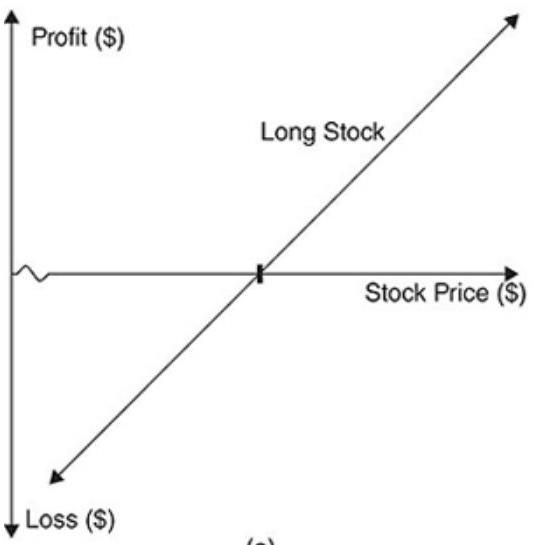
\includegraphics[max width=\textwidth]{2024_04_11_d71a2c9aea882dc3a7b2g-3(1)}
\end{center}

(a)

\begin{center}
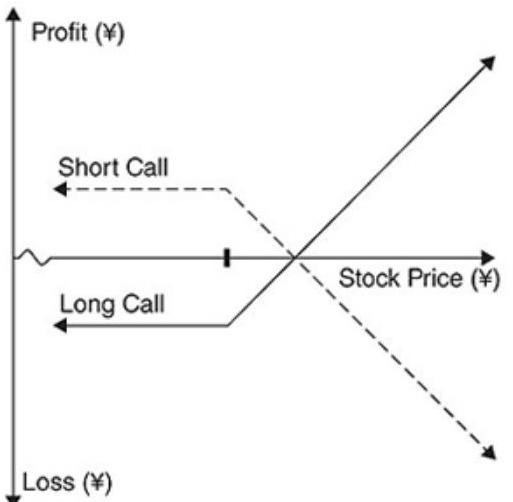
\includegraphics[max width=\textwidth]{2024_04_11_d71a2c9aea882dc3a7b2g-3(2)}
\end{center}

(c)

\begin{center}
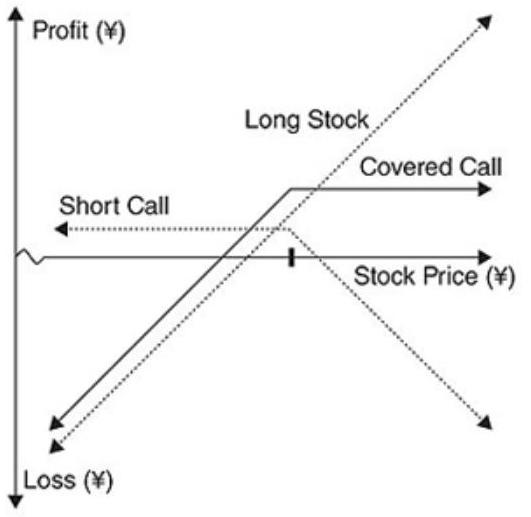
\includegraphics[max width=\textwidth]{2024_04_11_d71a2c9aea882dc3a7b2g-3(4)}
\end{center}

(e)

\begin{center}
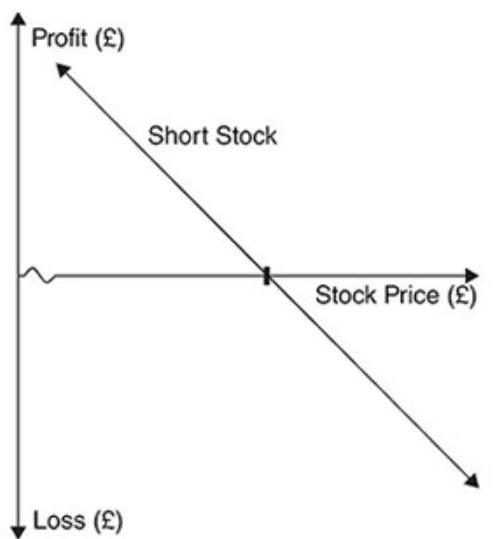
\includegraphics[max width=\textwidth]{2024_04_11_d71a2c9aea882dc3a7b2g-3(3)}
\end{center}

(b)

\begin{center}
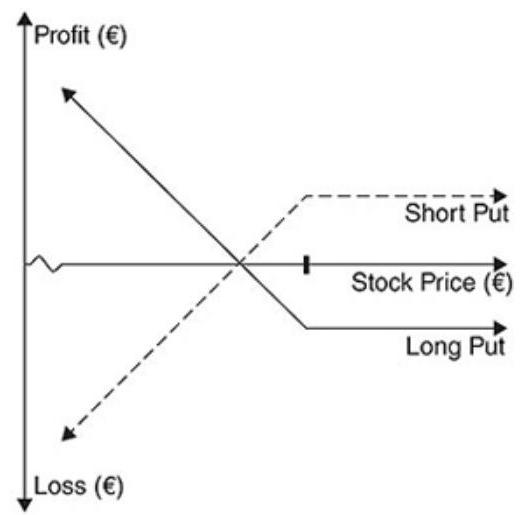
\includegraphics[max width=\textwidth]{2024_04_11_d71a2c9aea882dc3a7b2g-3}
\end{center}

(d)

\begin{center}
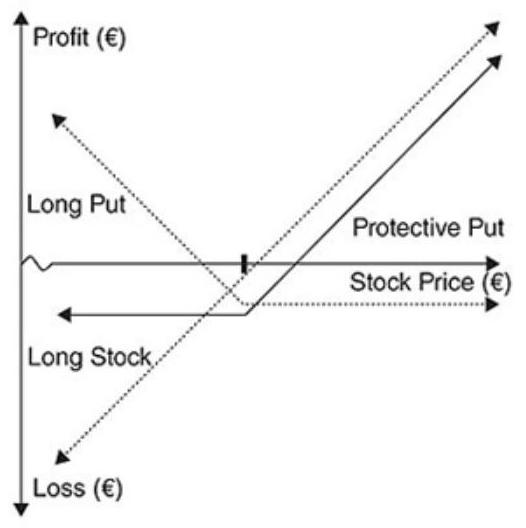
\includegraphics[max width=\textwidth]{2024_04_11_d71a2c9aea882dc3a7b2g-3(5)}
\end{center}

(f)

Diagrams of Underlying Assets and Simple Option Combinations

\section*{Call and Put Exposures}
The diagrams in the middle panel of the above exhibit illustrate the risk exposure of long and short positions in call options and put options. Both the short position and the long position are illustrated in the same diagram, with the short position denoted with a dashed line. Strike prices of the options are indicated with a mark on the horizontal axis. Whereas call options generate unlimited exposures to the upside of the underlying asset, put options do not have unlimited exposures in either direction, since the underlying asset's price cannot go below zero. Note that all kinks in option diagrams occur directly above or directly below the option's strike price. A short option position that is unhedged is often referred to as a naked option.

\section*{Covered Call and Protective Put Exposures}
The bottom panel of diagrams in the exhibit above illustrates the risk exposures of two popular combinations of an option and an underlying asset: a covered call and a protective put. A covered call combines being long an asset with being short a call option on the same asset. Note from the diagrams that a covered call has the same net risk exposure as a naked put.

A protective put combines being long an asset with a long position in a put option on the same asset. Note from the diagrams that a protective put has the same net risk exposure as a call option. The underlying components of the combinations are indicated with dotted lines, and the net exposure of the combination is indicated with a solid line.

\section*{FOUNDATION CHECK}
The material in this section and the diagrams in the exhibits assume familiarity with the netting of individual risk exposure diagrams to form diagrams of the net exposures of portfolios of options and/or underlying assets.

Both diagrams illustrate the put-call parity relationship among a call, a put, an underlying asset, and a zero-coupon default-free bond. Note that the diagram on the left illustrates that the risk exposure of an asset minus a call is equal to a short position in a put. The diagram on the right illustrates that the risk exposure of an asset plus a put is equal to a call. The zero-coupon default-free bond in the put-call parity relationship has no risk exposure but merely serves to balance the netted sizes of the positions. Put-call parity is discussed in the Put-Call Parity and Option Collars section.

\section*{Exposures of Two-Position Spreads}
The top panel of the next exhibit illustrates major option spreads, containing two positions each. An option spread (1) contains either call options or put options (not both), and (2) contains both long and short positions in options with the same underlying asset. Option spreads contain options that differ with regard to strike price, expiration date, or both. Option spreads based on differences only in expiration date are termed calendar spreads, or horizontal spreads. The illustrated option spreads differ only by strike price and are often referred to as vertical spreads. Diagonal spreads differ by both expiration date and strike price.\\
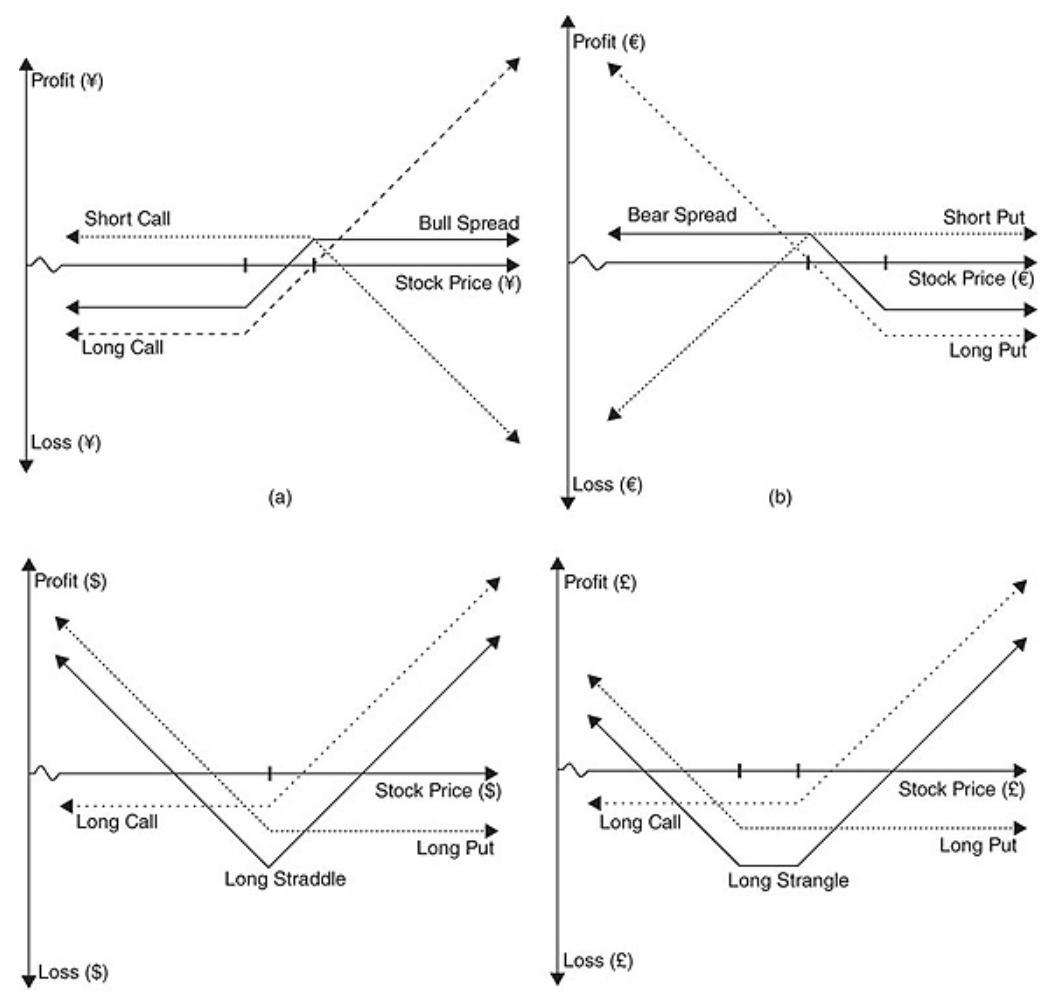
\includegraphics[max width=\textwidth, center]{2024_04_11_d71a2c9aea882dc3a7b2g-4(1)}

(c)

(d)\\
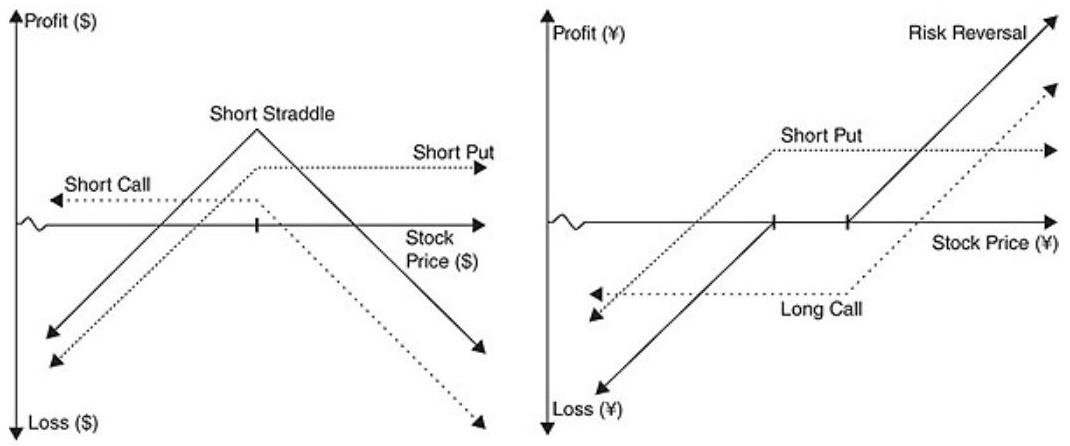
\includegraphics[max width=\textwidth, center]{2024_04_11_d71a2c9aea882dc3a7b2g-4}

(e)

(f)

\section*{Diagrams of Options Spreads and Combinations}
Consider a combination of one long position and one short position in either two calls or two puts that differ only by strike price. An option combination in which the long option position is at the lower of two strike prices is a bull spread, which offers bullish exposure to the underlying asset that begins at the lower strike price and ends at the higher strike price. The left side of the top panel of the exhibit above illustrates a bull spread. An option combination in which the long option position is at the higher of two strike prices is a bear spread, which offers bearish exposure to the underlying asset that begins at the higher strike price and ends at the lower strike price. The right side of the top panel of the exhibit above illustrates a bear spread. Note that bull spreads have long positions in the option with the lower strike price (and bear spreads have long positions in the option with the higher strike price) whether the spreads are formed with calls or with puts.

Spread positions termed ratio spreads can be formed in which the number of options in each position differ. For example, a ratio spread might contain two long call positions at one strike price and one short call position at another strike price, both with the same underlying asset. Ratio spreads tilt the option exposures to provide greater sensitivity (i.e., leverage) in one direction (e.g., bullish) than in the other. Spread ratios serve as an illustration of using greater degrees of leverage through establishing relatively large directional bets. The creation of positions that, over some ranges, are highly sensitive to changes in the value of the underlying asset is shown in the Credit Risk and Credit Derivatives session to be an important component of some structured products.

\section*{Exposures of Two-Position Combinations}
An option combination contains both calls and puts on the same underlying asset. The middle panel of Diagrams of Options Spreads and Combinations illustrates two major option combinations containing two positions each: option straddles and option strangles. An option straddle is a position in a call and put with the same sign (i.e., long or short), the same underlying asset, the same expiration date, and the same strike price. An option strangle is a position in a call and put with the same sign, the same underlying asset, the same expiration date, but different strike prices. When the call and put options are both long, the resulting position is a long straddle (or strangle); and when the call and put options are both short, the resulting position is a short straddle (or strangle). An option straddle is illustrated on the left side of the middle panel of Diagrams of Options Spreads and Combinations, and an option strangle is illustrated on the right side of the panel. The bottom left side of the above exhibit illustrates a short straddle.

The straddles and strangles discussed previously involved calls and puts with the same sign (i.e., long or short). Consider an option combination with a single call option and a single put option with the same underlying asset, the same time to expiration, but opposite signs. If the strike prices of the call and put are the same, the combination is a synthetic position in the underlying asset. If the call option is the long position and the put is short, the result is a synthetic long position in the underlying asset. If the call option is the short position and the put is long, the result is a synthetic short position in the underlying asset. By varying the strike prices of the options relative to the market price of the underlying asset, the synthetic positions can be designed to require no financing, to require some financing, or even to generate financing.

Consider a position similar to the previously discussed synthetic long position (long a call and short a put) but with different strike prices. A long out-of-the-money call combined with a short out-of-the-money put on the same asset and with the same expiration date is termed a risk reversal. The right side of the bottom panel of Diagrams of Options Spreads and Combinations depicts the risk exposure of a risk reversal. Note that the position resembles a synthetic long position except for the level range between the strike prices. Reversing the signs of the option positions (i.e., a short position in a risk reversal) generates a synthetic short position outside of the range between the strike prices.

There are specialized names for option combinations that have differently sized positions in puts and calls (e.g., straps and strips), which tilt the exposures to be more sensitive in one direction than the other. There are also positions of three or more options that are sometimes described with specialized terms, such as butterflies and condors. These more arcane terms are less frequently used in alternative investments.

\section*{Put-Call Parity and Option Collars}
In practice, the risk of an asset is often collared by buying a put option at strike price $K_{1}$ and writing a call option at strike price $K_{2}$ with $K_{1}<K_{2}$ to limit the range over which the investor is exposed to the risk of the underlying asset to movement of the underlying asset within the range between $K_{1}$ and $K_{2}$.

An option collar uses positions in options to limit the upside and downside exposure of a position to a price or rate, with the most common example being when the risk of a price or rate is limited by establishing a long position in a put option with a strike price $K_{1}$ and a short position in a call option with a strike price or rate of $K_{2}$ , in which $K_{1}<K_{2}$. The resulting position is collared and has the same net exposure of a bull call spread in in part (a) of the previous exhibit. A short position in a price or rate can be collared by a long position in a call option with a strike price $K_{1}$ and a short position in a put option with a strike price or rate of $K_{2}$, in which $K_{1}<K_{2}$. The resulting position is collared and has the same net exposure of a bear call spread in in part (b) of the previous exhibit.

One of the most important relationships within option analysis is put-call parity. Put-call parity is an arbitrage-free relation among the values of an asset, a riskless bond, a call option, and a put option. This relation was discussed briefly in the context of the previous exhibit. The options are European options on the same nondividend-paying underlying asset, with identical strike prices and expiration dates. The riskless bond is a zero-coupon default-free bond, with a face value equal to the strike price of the options and a maturity date equal to the expiration date of the options. Equation 1 illustrates one arrangement of put-call parity:


\begin{equation*}
\text { Call }+ \text { Bond }- \text { Put }=\text { Underlying Asset } \tag{1}
\end{equation*}


There are many ways to rearrange Equation 1 . As shown, the relation has the following intuition: A long position in both the call option and the bond, combined with a short position in the put option, will have the same value at the expiration date as a long position in the asset that underlies the options. The long call provides the upside exposure, and the short put provides the downside loss exposure. The riskless bond balances the amount of cash that must be invested when the positions are initiated (and will be received when the positions are terminated at the option expiration date). Since the left and right sides of the relation both have the same exposures and require the same investment, their values at all points in time must be the same in well-functioning capital markets.

Note also in Equation 1 that rearranging the equation to put both of the options on the right side generates the result that an asset combined with a long put position and short call position (with the same strike price) is equivalent to a zero-coupon bond. The long put and short call with the same strike price hedge all the risk from the underlying stock price at the option's expiration.


\end{document}